\documentclass[12pt,a4paper]{article}

% ---------- Fonts & language ----------
\usepackage{fontspec}
\usepackage{polyglossia}
\setdefaultlanguage{russian}
\setotherlanguage{english}
\setmainfont{Noto Sans}
\setsansfont{Noto Sans}
\usepackage{unicode-math}
\setmathfont{STIX Math}[Scale=1.38]

% ---------- Layout ----------
\usepackage[a4paper,top=14mm,bottom=14mm,left=16mm,right=16mm,headheight=5.3mm,headsep=6mm,footskip=9mm,includeheadfoot]{geometry}
\usepackage{microtype}
\usepackage{setspace}
\setstretch{1.06}
\usepackage{parskip}
\setlength{\parindent}{0pt}
\setlength{\parskip}{4pt}
\setlength{\emergencystretch}{1.5em}
\usepackage{enumitem}
\usepackage{needspace}
\setlist[itemize]{leftmargin=5.5mm,itemsep=1pt,topsep=2pt}
\setlist[enumerate]{leftmargin=7mm,itemsep=1pt,topsep=2pt}

% ---------- Math ----------
\usepackage{amsmath,mathtools}
\usepackage{array,tabularx,booktabs,multicol}
\newcommand{\dd}{\displaystyle}

% ---------- Graphs ----------
\usepackage{tikz}
\usetikzlibrary{arrows.meta,calc,positioning}
\usepackage{pgfplots}
\pgfplotsset{compat=1.18}

% ---------- Design ----------
\usepackage{xcolor}
\definecolor{MCBlue}{HTML}{007AFE}
\definecolor{MCDark}{HTML}{162033}
\definecolor{MCText}{HTML}{263247}
\definecolor{MCMid}{HTML}{6D7A90}
\definecolor{MCSoft}{HTML}{F1F8FF}
\definecolor{MCSoft2}{HTML}{F7FAFD}
\definecolor{MCPurple}{HTML}{7A3FF2}
\definecolor{MCGreen}{HTML}{10A66A}
\definecolor{MCRed}{HTML}{E44A5A}
\definecolor{MCGold}{HTML}{D99000}
\definecolor{MCGrid}{HTML}{D8E0EA}
\definecolor{MCAxis}{HTML}{596272}
\color{MCText}

\usepackage[most]{tcolorbox}
\tcbset{
  enhanced,
  boxrule=0pt,
  arc=3mm,
  outer arc=3mm,
  left=4mm,right=4mm,top=2.4mm,bottom=2.4mm,
  before skip=4pt,after skip=4pt,
}
\newtcolorbox{formulaBox}[1][]{colback=MCSoft,borderline west={1.8mm}{0pt}{MCBlue},#1}
\newtcolorbox{tipBox}[1][]{colback=MCSoft2,borderline west={1.5mm}{0pt}{MCGreen},#1}
\newtcolorbox{warnBox}[1][]{colback=MCRed!5,borderline west={1.5mm}{0pt}{MCRed},#1}
\newtcolorbox{quickBox}[1][]{colback=MCPurple!5,borderline west={1.5mm}{0pt}{MCPurple},#1}
\newtcolorbox{problemBox}[1][]{colback=MCSoft,borderline west={1.8mm}{0pt}{MCBlue},breakable,#1}
\newtcolorbox{countBox}[1][]{colback=MCPurple!4,borderline west={1.5mm}{0pt}{MCPurple},breakable,#1}
\newtcolorbox{answerBox}[1][]{colback=MCSoft,borderline west={1.8mm}{0pt}{MCBlue},breakable,#1}

% ---------- Headings ----------
\usepackage{titlesec}
\titleformat{\section}{\Large\bfseries\color{MCDark}}{\colorbox{MCBlue}{\textcolor{white}{\strut\hspace{2.6mm}\thesection\hspace{2.6mm}}}}{3mm}{}
\titlespacing*{\section}{0pt}{6pt}{4pt}
\titleformat{\subsection}{\large\bfseries\color{MCDark}}{}{0pt}{}
\titlespacing*{\subsection}{0pt}{5pt}{2pt}

% ---------- Header / footer ----------
\usepackage{fancyhdr}
\pagestyle{fancy}
\fancyhf{}
\fancyhead[L]{\small\color{MCMid}Параметры \textbullet\ Практика 1}
\fancyhead[R]{\href{https://vk.ru/vladislav_math}{\small\bfseries\color{MCBlue}Владислав Олегович}}
\fancyfoot[C]{\small\color{MCMid}\thepage}
\renewcommand{\headrulewidth}{0pt}
\renewcommand{\footrulewidth}{0pt}
\fancypagestyle{titlepage}{\fancyhf{}\fancyhead[R]{\href{https://vk.ru/vladislav_math}{\small\bfseries\color{MCBlue}Владислав Олегович}}\renewcommand{\headrulewidth}{0pt}\renewcommand{\footrulewidth}{0pt}}

% ---------- Links ----------
\usepackage{hyperref}
\hypersetup{colorlinks=true,linkcolor=MCBlue,urlcolor=MCBlue}

% ---------- Helpers ----------
\newcommand{\key}[1]{\textbf{\color{MCDark}#1}}
\newcommand{\eqv}{\;\Longleftrightarrow\;}
\newcommand{\imp}{\;\Longrightarrow\;}
\newcommand{\answer}[1]{\begin{answerBox}\textbf{\color{MCDark}Ответ:}~#1\end{answerBox}}
\newcommand{\legline}[2]{\tikz[baseline=-0.55ex]\draw[#1,line width=1.25pt] (0,0)--(7mm,0);\,#2}

\pgfplotsset{
  mcaxis/.style={
    axis lines=middle,
    axis line style={MCAxis,line width=.9pt},
    tick style={MCAxis},
    tick label style={font=\scriptsize,text=MCMid},
    label style={font=\small,text=MCAxis},
    major grid style={MCGrid,line width=.35pt},
    grid=major,
    enlargelimits=false,
    clip=true,
    samples=160,
    no markers,
    axis equal image
  }
}

\begin{document}

% ===================== TITLE =====================
\thispagestyle{titlepage}
\vspace*{8mm}
{\color{MCBlue}\rule{23mm}{2.2mm}}\\[8mm]
{\fontsize{32}{36}\selectfont\bfseries\color{MCDark}Параметры 1}\\[2mm]
{\fontsize{20}{24}\selectfont\color{MCBlue}\bfseries Практика}

\vspace{12mm}
{\Large\bfseries\color{MCDark}Карта занятия:}
\vspace{4mm}
\begin{tcolorbox}[colback=white,colframe=MCBlue!20,boxrule=.6pt,arc=4mm,left=6mm,right=6mm,top=6mm,bottom=6mm]
{\large\bfseries\color{MCBlue}Линейные функции}\par\vspace{3mm}
\begin{enumerate}[label={\color{MCBlue}\bfseries\arabic*.},leftmargin=9mm,itemsep=7pt]
  \item \key{Параллельный перенос}
  \item \key{Пучок прямых}
  \item \key{Система $xOa$}
\end{enumerate}
\end{tcolorbox}
\vfill
\newpage

% ===================== EXAMPLE 1 =====================
\Needspace{55mm}\section{Пример 1}
\begin{problemBox}
Найдите все значения параметра $a$, при каждом из которых система
\[
\begin{cases}
\dfrac{(y^2-xy+2x-2y)\sqrt{x+1}}{\sqrt{6-x}}=0,\\[2mm]
x+y-a-1=0
\end{cases}
\]
имеет ровно два различных решения.
\end{problemBox}

\subsection{Решение}
\begin{tipBox}
\[
\frac{A}{B}=0\eqv\begin{cases}A=0,\\B\ne0,\end{cases}
\qquad
\sqrt A\text{ существует}\eqv A\ge0,
\qquad
\frac1{\sqrt A}\text{ существует}\eqv A>0.
\]
\end{tipBox}

Рассмотрим первое уравнение системы:
\[
\begin{cases}
(y^2-xy+2x-2y)\sqrt{x+1}=0,\\
6-x>0.
\end{cases}
\]
\[
y^2-xy+2x-2y=(y-2)(y-x),
\qquad
(y-2)(y-x)\sqrt{x+1}=0.
\]
\[
6-x>0\eqv x<6,
\qquad
x+1\ge0\eqv x\ge-1.
\]
Следовательно,
\begin{formulaBox}
\[
\begin{cases}
-1\le x<6,\\[1mm]
\left[\begin{aligned}
y&=2,\\
y&=x,\\
x&=-1.
\end{aligned}\right.
\end{cases}
\]
\end{formulaBox}

Рассмотрим второе уравнение:
\[
x+y-a-1=0\eqv\boxed{y=-x+a+1}.
\]
Это прямая с угловым коэффициентом $k=-1$, проходящая через точку $(0;a+1)$.

\begin{center}
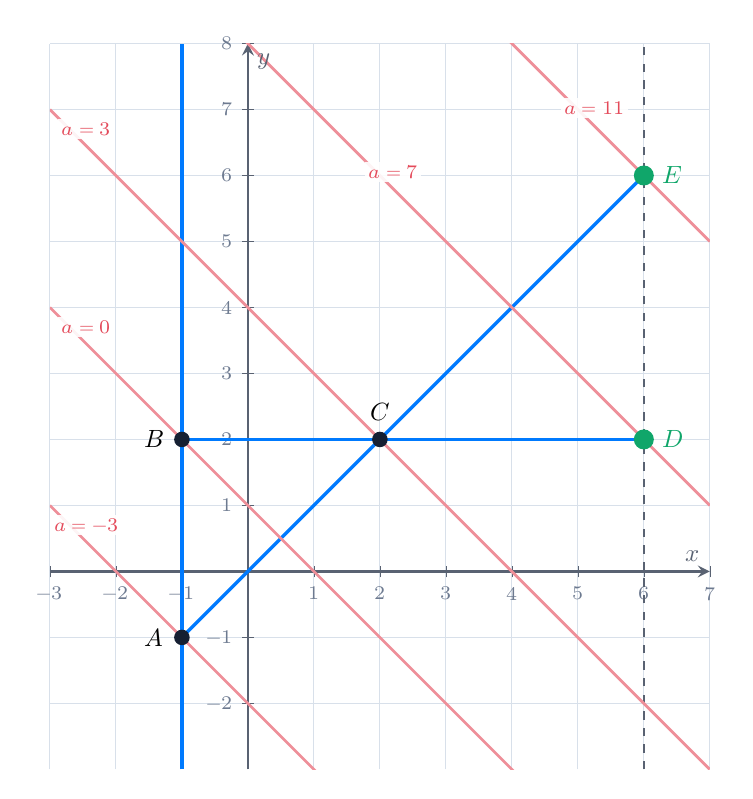
\begin{tikzpicture}
\begin{axis}[
  mcaxis,width=.95\textwidth,height=108mm,
  xmin=-3,xmax=7,ymin=-3,ymax=8,
  xtick={-3,-2,-1,0,1,2,3,4,5,6,7},
  ytick={-2,-1,0,1,2,3,4,5,6,7,8},
  xlabel={$x$},ylabel={$y$}
]
\addplot[MCBlue,very thick,domain=-1:5.995] {2};
\addplot[MCBlue,very thick,domain=-1:5.995] {x};
\addplot[MCBlue,very thick] coordinates {(-1,-3) (-1,8)};
\addplot[MCAxis,dashed,line width=.9pt] coordinates {(6,-3) (6,8)};
\addplot[MCRed!62,line width=1pt,domain=-3:7] {-x-2};
\addplot[MCRed!62,line width=1pt,domain=-3:7] {-x+1};
\addplot[MCRed!62,line width=1pt,domain=-3:7] {-x+4};
\addplot[MCRed!62,line width=1pt,domain=-3:7] {-x+8};
\addplot[MCRed!62,line width=1pt,domain=-3:7] {-x+12};
\addplot[only marks,mark=*,mark size=2.6pt,MCDark] coordinates {(-1,-1) (-1,2) (2,2)};
\addplot[only marks,mark=o,mark size=3pt,MCGreen,very thick] coordinates {(6,2) (6,6)};
\node[font=\small\bfseries,anchor=east] at (axis cs:-1.14,-1) {$A$};
\node[font=\small\bfseries,anchor=east] at (axis cs:-1.14,2) {$B$};
\node[font=\small\bfseries,anchor=south] at (axis cs:2,2.13) {$C$};
\node[font=\small\bfseries,text=MCGreen,anchor=west] at (axis cs:6.14,2) {$D$};
\node[font=\small\bfseries,text=MCGreen,anchor=west] at (axis cs:6.14,6) {$E$};
\node[font=\scriptsize\bfseries,text=MCRed,fill=white,fill opacity=.9,text opacity=1,inner sep=1.2pt] at (axis cs:-2.45,.70) {$a=-3$};
\node[font=\scriptsize\bfseries,text=MCRed,fill=white,fill opacity=.9,text opacity=1,inner sep=1.2pt] at (axis cs:-2.45,3.70) {$a=0$};
\node[font=\scriptsize\bfseries,text=MCRed,fill=white,fill opacity=.9,text opacity=1,inner sep=1.2pt] at (axis cs:-2.45,6.70) {$a=3$};
\node[font=\scriptsize\bfseries,text=MCRed,fill=white,fill opacity=.9,text opacity=1,inner sep=1.2pt] at (axis cs:2.20,6.05) {$a=7$};
\node[font=\scriptsize\bfseries,text=MCRed,fill=white,fill opacity=.9,text opacity=1,inner sep=1.2pt] at (axis cs:5.25,7.02) {$a=11$};
\end{axis}
\end{tikzpicture}

\smallskip
\begin{tabular}{c@{\hspace{6mm}}c@{\hspace{6mm}}c}
\legline{MCBlue}{фиксированный график} &
\legline{MCRed!62}{подвижная $y=-x+a+1$} &
\legline{MCAxis,dashed}{граница $x=6$}
\end{tabular}

{\small\color{MCMid}Критические положения: $a=-3,\ 0,\ 3,\ 7,\ 11$.}
\end{center}

Найдём значения параметра у прямой $y=-x+a+1$, проходящей через критические точки:
\[
\begin{aligned}
A(-1;-1):&\quad -1=1+a+1 &&\imp a=-3,\\
B(-1;2):&\quad 2=1+a+1 &&\imp a=0,\\
C(2;2):&\quad 2=-2+a+1 &&\imp a=3,\\
D(6;2):&\quad 2=-6+a+1 &&\imp a=7,\\
E(6;6):&\quad 6=-6+a+1 &&\imp a=11.
\end{aligned}
\]

\begin{countBox}
\renewcommand{\arraystretch}{1.18}
\begin{tabularx}{\textwidth}{>{\centering\arraybackslash}m{44mm}>{\centering\arraybackslash}X}
\textbf{Значение параметра} & \textbf{Число решений}\\ \midrule
$a\le-3$ & 1\\
$-3<a\le0$ & 2\\
$0<a<3$ & 3\\
$a=3$ & 2\\
$3<a<7$ & 3\\
$7\le a<11$ & 2\\
$a\ge11$ & 1
\end{tabularx}
\end{countBox}
\answer{$a\in(-3;0]\cup\{3\}\cup[7;11)$.}

% ===================== EXAMPLE 2 =====================
\Needspace{62mm}\section{Пример 2}
\begin{problemBox}
Найдите все значения параметра $a$, при каждом из которых система
\[
\begin{cases}
y^2-10y-x^2+6x+16=0,\\
y-ax=1,\\
x>1
\end{cases}
\]
имеет единственное решение.
\end{problemBox}

\subsection{Решение}
\[
y^2-10y+25=(y-5)^2,
\qquad
x^2-6x+9=(x-3)^2.
\]
Рассмотрим первое уравнение:
\[
y^2-10y+25-x^2+6x-9=0,
\]
\[
(y-5)^2-(x-3)^2=0,
\]
\[
(y-5-(x-3))(y-5+(x-3))=0.
\]
Следовательно,
\begin{formulaBox}
\[
\left[\begin{aligned}
y&=x+2,\\
y&=-x+8.
\end{aligned}\right.
\]
\end{formulaBox}

Рассмотрим второе уравнение:
\[
y-ax=1\eqv\boxed{y=ax+1}.
\]
Система имеет вид
\[
\begin{cases}
\left[\begin{aligned}
y&=x+2,\\
y&=-x+8,
\end{aligned}\right.\\[1mm]
y=ax+1,\\
x>1.
\end{cases}
\]

\begin{center}
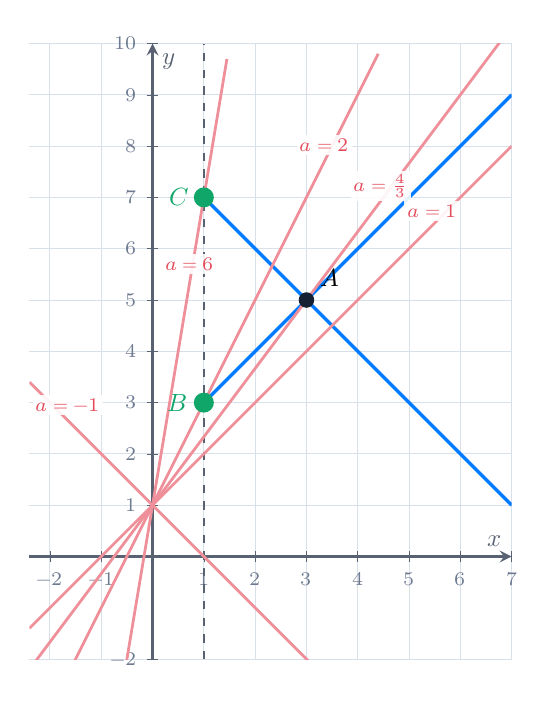
\begin{tikzpicture}
\begin{axis}[
  mcaxis,width=.84\textwidth,height=94mm,
  xmin=-2.4,xmax=7,ymin=-2,ymax=10,
  xtick={-2,-1,0,1,2,3,4,5,6,7},
  ytick={-2,0,1,2,3,4,5,6,7,8,9,10},
  xlabel={$x$},ylabel={$y$}
]
\addplot[MCBlue,very thick,domain=1.005:7] {x+2};
\addplot[MCBlue,very thick,domain=1.005:7] {-x+8};
\addplot[MCAxis,dashed,line width=.9pt] coordinates {(1,-2) (1,10)};
\addplot[MCRed!62,line width=1pt,domain=-2.4:7] {-x+1};
\addplot[MCRed!62,line width=1pt,domain=-2.4:7] {x+1};
\addplot[MCRed!62,line width=1pt,domain=-2.4:7] {4*x/3+1};
\addplot[MCRed!62,line width=1pt,domain=-2.4:4.4] {2*x+1};
\addplot[MCRed!62,line width=1pt,domain=-1.6:1.45] {6*x+1};
\addplot[only marks,mark=o,mark size=3pt,MCGreen,very thick] coordinates {(1,3) (1,7)};
\addplot[only marks,mark=*,mark size=2.6pt,MCDark] coordinates {(3,5)};
\node[font=\small\bfseries,text=MCGreen,anchor=east] at (axis cs:.86,3) {$B$};
\node[font=\small\bfseries,text=MCGreen,anchor=east] at (axis cs:.86,7) {$C$};
\node[font=\small\bfseries,anchor=south west] at (axis cs:3.08,5.08) {$A$};
\node[font=\scriptsize\bfseries,text=MCRed,fill=white,fill opacity=.9,text opacity=1,inner sep=1.2pt] at (axis cs:-1.65,2.95) {$a=-1$};
\node[font=\scriptsize\bfseries,text=MCRed,fill=white,fill opacity=.9,text opacity=1,inner sep=1.2pt] at (axis cs:5.45,6.73) {$a=1$};
\node[font=\scriptsize\bfseries,text=MCRed,fill=white,fill opacity=.9,text opacity=1,inner sep=1.2pt] at (axis cs:4.45,7.22) {$a=\frac43$};
\node[font=\scriptsize\bfseries,text=MCRed,fill=white,fill opacity=.9,text opacity=1,inner sep=1.2pt] at (axis cs:3.35,8.02) {$a=2$};
\node[font=\scriptsize\bfseries,text=MCRed,fill=white,fill opacity=.9,text opacity=1,inner sep=1.2pt] at (axis cs:.72,5.70) {$a=6$};
\end{axis}
\end{tikzpicture}

\smallskip
\begin{tabular}{c@{\hspace{6mm}}c@{\hspace{6mm}}c}
\legline{MCBlue}{фиксированные прямые} &
\legline{MCRed!62}{$y=ax+1$} &
\legline{MCAxis,dashed}{$x=1$}
\end{tabular}

{\small\color{MCMid}Критические значения: $a=-1,\ 1,\ \frac43,\ 2,\ 6$.}
\end{center}

Определим критические значения параметра:
\[
\begin{aligned}
1)&\quad y=ax+1\parallel y=-x+8 &&\imp a=-1,\\
2)&\quad y=ax+1\parallel y=x+2 &&\imp a=1,\\
3)&\quad A:\ x+2=-x+8\imp x=3,\ y=5,\\
&\qquad 5=3a+1 &&\imp a=\frac43,\\
4)&\quad B(1;3):\quad 3=a+1 &&\imp a=2,\\
5)&\quad C(1;7):\quad 7=a+1 &&\imp a=6.
\end{aligned}
\]

\begin{countBox}
\renewcommand{\arraystretch}{1.18}
\begin{tabularx}{\textwidth}{>{\centering\arraybackslash}m{44mm}>{\centering\arraybackslash}X}
\textbf{Значение параметра} & \textbf{Число решений}\\ \midrule
$a\le-1$ & 0\\
$-1<a\le1$ & 1\\
$1<a<\frac43$ & 2\\
$a=\frac43$ & 1\\
$\frac43<a<2$ & 2\\
$2\le a<6$ & 1\\
$a\ge6$ & 0
\end{tabularx}
\end{countBox}
\answer{$a\in(-1;1]\cup\left\{\frac43\right\}\cup[2;6)$.}

% ===================== EXAMPLE 3 =====================
\Needspace{58mm}\section{Пример 3}
\begin{problemBox}
Найдите все значения параметра $a$, при каждом из которых уравнение
\[
\frac{4x^2-a^2}{x^2+6x+9-a^2}=0
\]
имеет единственное решение.
\end{problemBox}

\subsection{Решение}
\[
\frac AB=0\eqv\begin{cases}A=0,\\B\ne0.\end{cases}
\]
\[
\begin{cases}
4x^2-a^2=0,\\
x^2+6x+9-a^2\ne0
\end{cases}
\eqv
\begin{cases}
(2x-a)(2x+a)=0,\\
(x+3-a)(x+3+a)\ne0.
\end{cases}
\]
Перейдём к системе координат $xOa$:
\begin{formulaBox}
\[
\begin{cases}
\left[\begin{aligned}
a&=2x,\\
a&=-2x,
\end{aligned}\right.\\[1mm]
a\ne x+3,\\
a\ne -x-3.
\end{cases}
\]
\end{formulaBox}

\begin{center}
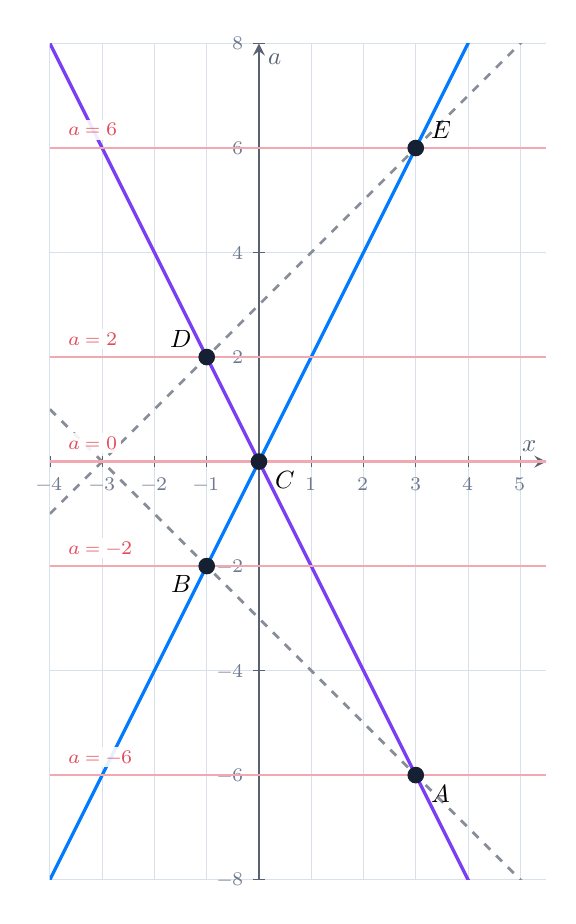
\begin{tikzpicture}
\begin{axis}[
  mcaxis,width=.84\textwidth,height=122mm,
  xmin=-4,xmax=5.5,ymin=-8,ymax=8,
  xtick={-4,-3,-2,-1,0,1,2,3,4,5},
  ytick={-8,-6,-4,-2,0,2,4,6,8},
  xlabel={$x$},ylabel={$a$}
]
\addplot[MCBlue,very thick,domain=-4:5.5] {2*x};
\addplot[MCPurple,very thick,domain=-4:5.5] {-2*x};
\addplot[MCAxis!72,dashed,line width=1pt,domain=-4:5.5] {x+3};
\addplot[MCAxis!72,dashed,line width=1pt,domain=-4:5.5] {-x-3};
\foreach \yy in {-6,-2,0,2,6}{\addplot[MCRed!48,line width=.8pt,domain=-4:5.5] {\yy};}
\addplot[only marks,mark=*,mark size=2.8pt,MCDark] coordinates {(3,-6) (-1,-2) (0,0) (-1,2) (3,6)};
\node[font=\small\bfseries,anchor=north west] at (axis cs:3.12,-6) {$A$};
\node[font=\small\bfseries,anchor=north east] at (axis cs:-1.12,-2) {$B$};
\node[font=\small\bfseries,anchor=north west] at (axis cs:.12,0) {$C$};
\node[font=\small\bfseries,anchor=south east] at (axis cs:-1.12,2) {$D$};
\node[font=\small\bfseries,anchor=south west] at (axis cs:3.12,6) {$E$};
\node[font=\scriptsize\bfseries,text=MCRed,fill=white,fill opacity=.9,text opacity=1,inner sep=1.2pt,anchor=west] at (axis cs:-3.72,-5.65) {$a=-6$};
\node[font=\scriptsize\bfseries,text=MCRed,fill=white,fill opacity=.9,text opacity=1,inner sep=1.2pt,anchor=west] at (axis cs:-3.72,-1.65) {$a=-2$};
\node[font=\scriptsize\bfseries,text=MCRed,fill=white,fill opacity=.9,text opacity=1,inner sep=1.2pt,anchor=west] at (axis cs:-3.72,.35) {$a=0$};
\node[font=\scriptsize\bfseries,text=MCRed,fill=white,fill opacity=.9,text opacity=1,inner sep=1.2pt,anchor=west] at (axis cs:-3.72,2.35) {$a=2$};
\node[font=\scriptsize\bfseries,text=MCRed,fill=white,fill opacity=.9,text opacity=1,inner sep=1.2pt,anchor=west] at (axis cs:-3.72,6.35) {$a=6$};
\end{axis}
\end{tikzpicture}

\smallskip
\begin{tabular}{c@{\hspace{5mm}}c}
\legline{MCBlue}{$a=2x$} & \legline{MCPurple}{$a=-2x$}\\[1mm]
\legline{MCAxis,dashed}{$a=x+3,\ a=-x-3$} & \legline{MCRed!48}{уровни $a=-6,-2,0,2,6$}
\end{tabular}
\end{center}

Найдём координаты критических точек:
\[
\begin{aligned}
A:&\quad a=-2x,\ a=-x-3 &&\imp -2x=-x-3\imp x=3,\ a=-6,\\
B:&\quad a=2x,\ a=-x-3 &&\imp 2x=-x-3\imp x=-1,\ a=-2,\\
C:&\quad a=2x,\ a=-2x &&\imp x=0,\ a=0,\\
D:&\quad a=-2x,\ a=x+3 &&\imp -2x=x+3\imp x=-1,\ a=2,\\
E:&\quad a=2x,\ a=x+3 &&\imp 2x=x+3\imp x=3,\ a=6.
\end{aligned}
\]

\begin{quickBox}
Одно решение получается при
\[
a\in\{-6;-2;0;2;6\}.
\]
\end{quickBox}
\answer{$a\in\{-6;-2;0;2;6\}$.}

\end{document}
